\documentclass{ethz_report}
\usepackage{listings}
\usepackage{color}
\usepackage{caption}
\usepackage{subcaption}


\definecolor{codegreen}{rgb}{0,0.6,0}
\definecolor{codegray}{rgb}{0.5,0.5,0.5}
\definecolor{codepurple}{rgb}{0.58,0,0.82}
\definecolor{backcolour}{rgb}{1,1,1}

\lstdefinestyle{mystyle}{
    backgroundcolor=\color{backcolour},
    commentstyle=\color{codegreen},
    keywordstyle=\color{magenta},
    numberstyle=\tiny\color{codegray},
    stringstyle=\color{codepurple},
    basicstyle=\ttfamily,
    breakatwhitespace=false,
    breaklines=true,
    captionpos=b,
    keepspaces=true,
    numbers=left,
    numbersep=5pt,
    showspaces=false,
    showstringspaces=false,
    showtabs=false,
    tabsize=4,
    frame=lines
}
\lstset{style=mystyle}

\title{Exercise 5 - Shape from Silhouettes}
\subject{Computer Vision}
\author{Alberto Montes}
\email{malberto@student.ethz.ch}
\date{\today}

\begin{document}
\maketitle

\section*{Silhouette extraction}

The first task consists on setting the best threshold to extract the image silhouette. With the given images, the best threshold found was $100$ which extract all the figure including the darkest zones because of shadows. It also extract some other places of the environment, but with the bounding box, the noisy extracted parts disappear. On Figure~\ref{fig:silhouette_extraction} there a snapshot of the silhouette extraction.

\begin{figure}[H]
    \centering
    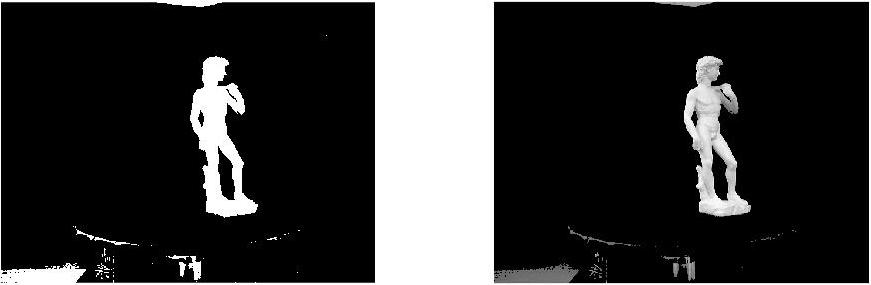
\includegraphics[width=1\linewidth]{images/silhouette_extraction}
    \caption{Silhouette extraction}
    \label{fig:silhouette_extraction}
\end{figure}

\section*{Volume of interest}

Once the silhouette is extracted, it is required to specify the bounding box that will define the volume of interest for the computation of the Visual Hull.
After some iterations, the final values for the bounding box to fit the object has been:

\begin{equation}
    \begin{bmatrix}
        x_{min} & y_{min} & z_{min} \\
        x_{max} & y_{max} & z_{max}
    \end{bmatrix}
    =
    \begin{bmatrix}
        0 & -0.5 & -2 \\
        2.5 & 2 & 3
    \end{bmatrix}
\end{equation}

On Figure~\ref{fig:volume_of_interest} there is a snapshot of the bounding box represented over the silhouette.

\begin{figure}[H]
    \centering
    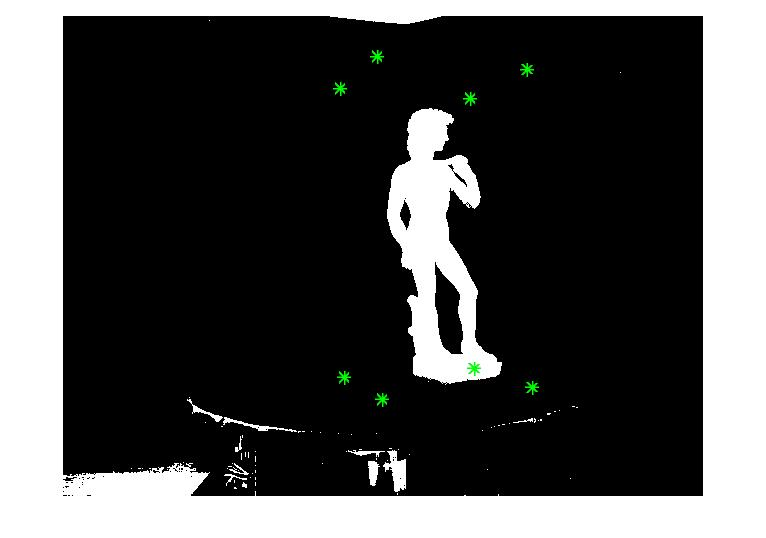
\includegraphics[width=.5\linewidth]{images/volume_of_interest}
    \caption{Volume of Interest}
    \label{fig:volume_of_interest}
\end{figure}

\section*{Visual Hull}

The final step to achieve a 3D reconstruction of the original object at the images, is to compute the Visual Hull. To do so, it has been divided 



\lstinputlisting[language=MATLAB, caption=computeVisualHull, firstline=79, lastline=103, label={lst:compute_visual_hull}]{../code/exercise5.m}


\begin{figure}[H]
\centering
\begin{subfigure}[b]{.5\textwidth}
  \centering
  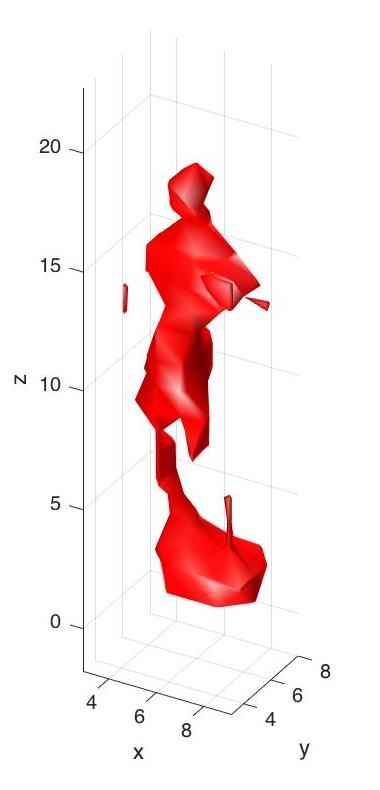
\includegraphics[width=.8\linewidth]{images/visual_hull_low}
  \caption{Volume size: $(10, 10, 20)$}
\end{subfigure}%
\begin{subfigure}[b]{.5\textwidth}
  \centering
  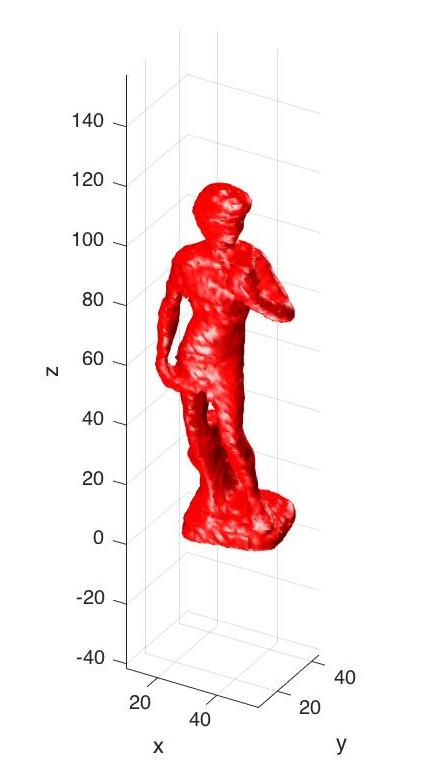
\includegraphics[width=.8\linewidth]{images/visual_hull_high}
  \caption{Volume size: $(64, 64, 128)$}
\end{subfigure}
\caption{Volume Hull for different resolutions}
\label{fig:fun_mat}
\end{figure}


\section*{Improvements}


\end{document}
